\section{Experiments}
\label{sec:experiments}

In this section, we present experiments conducted on randomly generated task sets. Five schedulability tests for dynamic self-suspending tasks are compared, namely, the suspension oblivious approach (Section~\ref{sec:suspension-oblivious}), the modeling of suspension as a release jitter (Section~\ref{sec:jitter}), the analysis proposed by Jane W.S. Liu and proven correct in this paper that models the suspension as blocking (Section~\ref{sec:suspension-blocking}), the generic framework of Corollary~\ref{corollary:general-framework} (called ECRTS 16 in the plots) and the test based on the linear approximation presented in Section~\ref{sec:linear-approximation} (called ECRTS 16 linear in the plots) . In those experiments, the tasks are assumed to be scheduled with rate monotonic and have implicit deadlines (i.e., $D_i = T_i$).

The task sets were generated using the \texttt{randfixedsum} algorithm presented in \cite{Emberson-taskSetGeneration-2010}. Let $C'_i$ denote the sum of $C_i$ and $S_i$ (i.e., $C'_i \equals C_i + S_i$). That is, $C'_i$ is the WCET of a task for which the suspension time would be considered as execution time like it is the case in the test of Section~\ref{sec:suspension-oblivious}. The modified utilization of $\tau_i$ is then given by $U'_i \equals \frac{C'_i}{T_i}$ and the total modified utilization is $U' \equals \sum_{i=1}^n U'_i$. The task generator uses the \texttt{randfixedsum} algorithm to generate $n$ values $U'_i$ (one for each task) with total modified utilization $U'$. A period $T_i$ is then randomly generated from a uniform distribution spanning from $100$ to $10000$. The resulting value $C'_i = U'_i \times T_i$ is then divided in the two components $C_i$ and $S_i$ using a random ratio $r_i$ obtained from a uniform distribution between a value $r_{\min}$ and $r_{\max}$ depending of the specific experiment performed. That is, $S_i \equals r_i \times C'_i$ and $C_i = (1 - r_i) \times C'_i$. 

\begin{figure*}[t!]
  \centering
  \subfloat[Varying the number of tasks $n$, $U'=0.95$, $r_{\min} = 0.05$, $r_{\max} = 0.5$]{\label{fig:plot1} 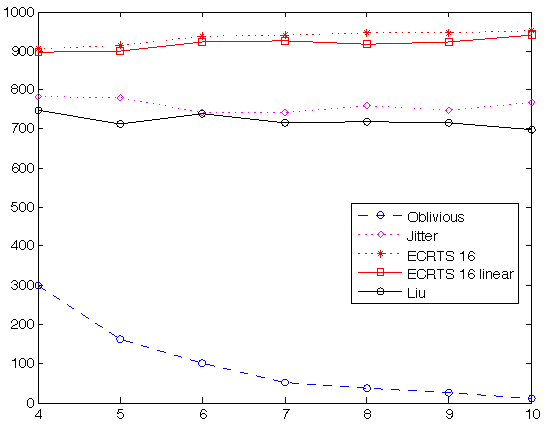
\includegraphics[width=0.4\textwidth]{../figures/experiments/varyingn_smin=5_smax=50_U=0_95_T=100-10000_1000runs_croped.pdf}}
  \subfloat[Varying $r_{\max}$, $U'=1$, $n=8$, $r_{\min} = 0.05$]{\label{fig:plot2} 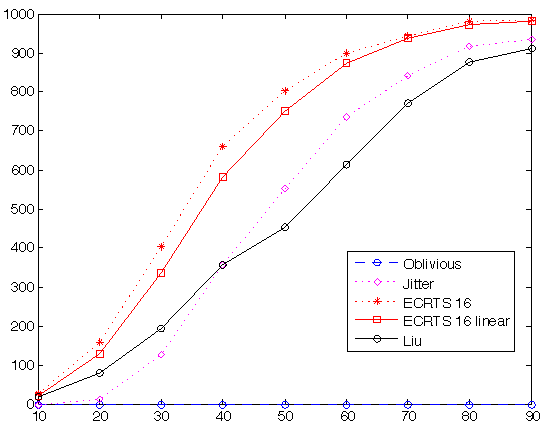
\includegraphics[width=0.4\textwidth]{../figures/experiments/varyingSmax_smin=5_U=1_n=8_T=100-10000_1000runs_croped.pdf}}\\ 
  \subfloat[Varying $U'$, $n=8$, $r_{\min} = 0.05$, $r_{\max} = 0.5$]{\label{fig:plot3} 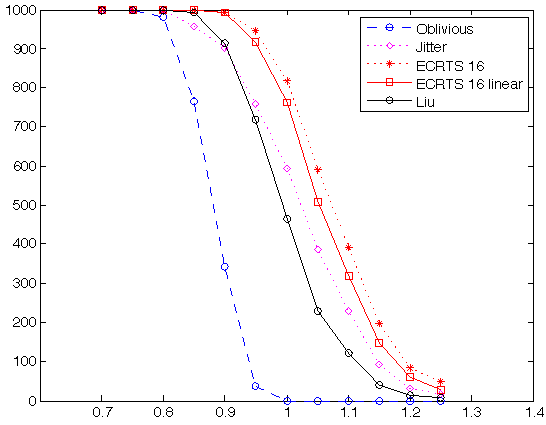
\includegraphics[width=0.4\textwidth]{../figures/experiments/varyingU_smin=5_smax=50_n=8_T=100-10000_1000runs_croped.pdf}}
  \subfloat[Varying $U'$, $n=8$, $r_{\min} = 0.5$, $r_{\max} = 0.9$]{\label{fig:plot4} 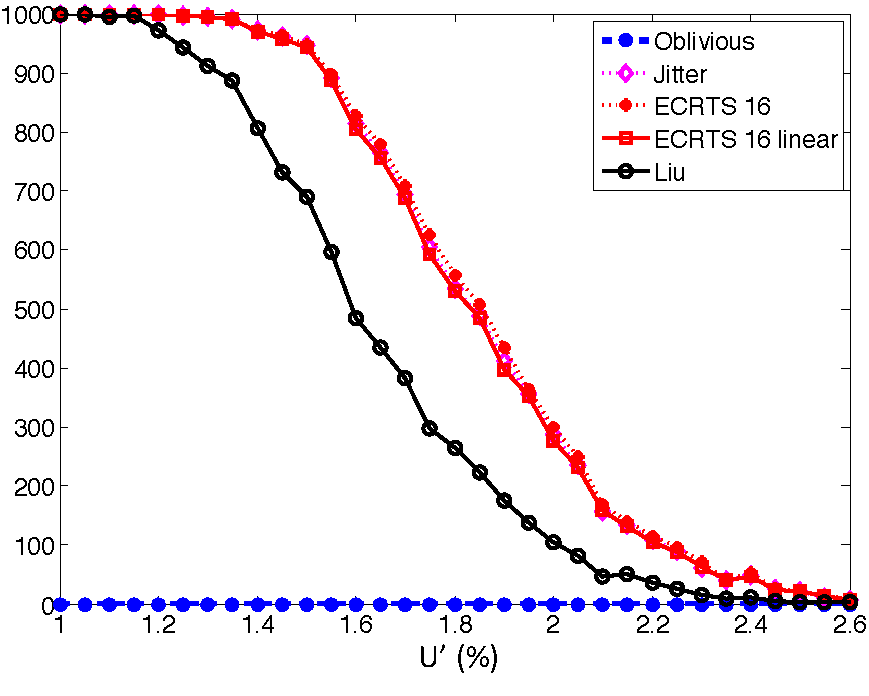
\includegraphics[width=0.4\textwidth]{../figures/experiments/varyingU_smin=50_smax=90_n=8_T=100-10000_1000runs_croped.pdf}} 
  \caption{Number of schedulable task sets over $1000$ randomly generated task sets.}
  \label{fig:exp}
\end{figure*}

Each point in the plots of Figure~\ref{fig:exp} represents the number of task sets that were deemed schedulable by the respective algorithm over $1000$ different experiments.

Four different types of experiments are reported in this paper. The first one is presented in Figure~\ref{fig:plot1}. It presents the evolution of the number of task sets deemed schedulable when the number of self-suspending tasks increases. The number of tasks $n$ is varied from $4$ to $10$ for a total modified utilization $U'$ of $0.95$. As can be seen in Figure~\ref{fig:plot1}, at the exception of the suspension oblivious analysis, the performances of the tests are barely influenced by the number of fact. In fact, the number of task sets found schedulable by the test of Corollary~\ref{corollary:general-framework} and the linear test of Section~\ref{sec:linear-approximation} slightly increases with the number of tasks. It is the opposite behavior than the suspension oblivious approach. One can already conclude from this plot that the tests developed in this paper perform way better than the state-of-the-art. Furthermore, the difference between the performances of the complete test of Corollary~\ref{corollary:general-framework} and its linear version are quite small, thereby making the linear test a practical and useful analysis.

The second experiment is presented in Figure~\ref{fig:plot2} and shows the evolution of the performances of the tests with respect to the length of the total suspension time of a task when the total modified utilization $U'$ and the number of tasks are kept constant. The value of $r_{\max}$ is then varied from $10\%$ to $90\%$, hence increasing the number of tasks with high suspension times. The value $r_{\min}$ is kept constant at $5\%$, so as to keep a certain diversity in the suspension behavior of each task. As expected, the suspension oblivious approach does not accept any task set since the total modified utilization is equal to $100\%$. For the other tests however, the number of schedulable task sets increases when the suspension times become larger. Indeed, the actual workload, which accounts only for the WCET $C_i$, decreases when $S_i$ increases. Again, one can see the improvement of the tests of this paper over the state-of-the-art. Interestingly, one can also witnesses the incomparability of the jitter based and the blocking based schedulability tests. The jitter based test performs better for large blocking times while the blocking based test has better results for lower blocking times.

The last two plots (Figures~\ref{fig:plot3} and~\ref{fig:plot4}), present the results obtained when the total modified utilization increases but the distribution of suspension times and the number of tasks remain identical. As expected, the number of schedulable task sets decreases when the utilization increases. Again, the incomparability of the jitter- and blocking-based tests can be seen. The test based on blocking usually performs better for lower utilizations. The improvement of Corollary~\ref{corollary:general-framework} over the state-of-the-art is still high when suspension times are in average smaller than the execution times of the tasks (see Figures~\ref{fig:plot3}). However, when the suspension time becomes larger than the execution time of the task (see Figures~\ref{fig:plot4}), the release jitter-based test performs almost as well as Corollary~\ref{corollary:general-framework}.
